\chapter{Experiments} \label{chapter:experiments}
In this section we will cover the process of preparing the collected dataset, described in section \ref{chapter:datacollection} and training different types of tokenizers and language models until we found the best performing one.

\section{Tokenization of the dataset}
In order to use the dataset created earlier in the chapter \ref{chapter:datacollection} for the BERT based model as training input, it must be transformed into a suitable format. Since we are using the Huggingface trainer, we also need to follow the Huggingface training data format. \newline
In the first step, the entire text from the CSV file is converted into a dataset dictionary. This is possible with one line of code after importing the datasets package.

\begin{code}
\captionof{listing}{Creating the Dataset Dictionary}
\label{code:dict}
\begin{minted}{python}
from datasets import Dataset
training_data = Dataset.from_dict(df)
datasets = datasets.DatasetDict({"train": train_data})
	\end{minted}
\end{code}

When using this method, training and test data can be stored together in one object and accessed via the datasets["train"] or datasets["test"] index. The resulting datasets["train"] dictionary has the feature "text" to access the data and 1.052.587 rows as visible in the output depicted in Figure \ref{fig:dict_features}.
\begin{figure}[H]
	\centering
	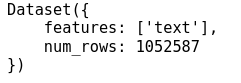
\includegraphics[width=0.4\textwidth]{figures/dataset_dict_features.png}
	\caption{Format of Dataset Dictionary}
	\label{fig:dict_features}
\end{figure}

The next step is to apply the tokenizer to the entire text. For this we use the map method from the datasets library. First we define a method shown in Listing \ref{code:tok_funct} which calls the tokenizer on the text.

\begin{code}
	\captionof{listing}{Tokenize Function to call on the text}
	\label{code:tok_funct}
	\begin{minted}{python}
def tokenize_function(examples):
return tokenizer(examples["text"])
	\end{minted}
\end{code}

The map function, shown in Listing \ref{code:tok_map}, can be used to apply the tokenizer function from Listing \ref{code:tok_funct} to the entire dataset. To speed up the process, we pass the number\_poc=4 attribute, which enables multithreading and splits the process into four threads.

\begin{code}
	\captionof{listing}{Applying the tokenize function on the Text}
	\label{code:tok_map}
	\begin{minted}{python}
tokenized_datasets = datasets.map(tokenize_function, batched=True, num_proc=4, 
	remove_columns=["text"])
	\end{minted}
\end{code}

The "text" collumn from the dictionary has now been replaced by the input\_ids which is needed by the modell as an input for training.

\begin{figure}[H]
	\centering
	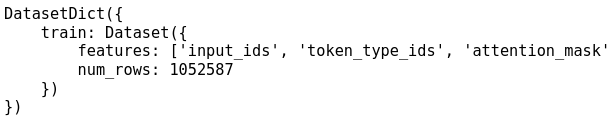
\includegraphics[width=0.8\textwidth]{figures/tok_dataset.png}
	\caption{Text collumn has been replaced by calling tokenizer on the dataset.}
	\label{fig:dict_tokenized}
\end{figure}

After the dataset has been tokenized, the next step is to split it into individual chunks. The size of these chunks depends on the available resources and the maximum context size of the model. The context size can be determined with the method \alert{model\_max\_length}. For BERT based models, like ours, it is 512 tokens.
We need to concatenate all of our texts together and then split the result in small chunks of a certain \alert{chunk\_size}. To do this, we will use the \alert{map} method again, with the option \alert{batched=True}. This option actually lets us change the number of examples in the datasets by returning a different number of examples than we got. This way, we can create our new samples from a batch of examples.\newline
First, we grab the maximum length our model was pretrained with. This might be a big too big to fit in our GPU RAM. In the first try we chose a chunk size of 64, which turned out not to be suitable because longer sentences were truncated, while shorter sentences were populated with [PAD] tokens (id: 0) until they reach the desired length. Using a small chunk size can be detrimental in real-world scenarios, so it is recommended to use a size that corresponds to the use case the model will be applied to. Because of that we chose a chunk size of 128.

\begin{code}
	\captionof{listing}{Definition of the method group\_text}
	\label{code:group_text}
	\begin{minted}{python}
chunk_size = 128

def group_texts(examples):
# Concatenate all texts
concatenated_examples = {k: sum(examples[k], []) for k in examples.keys()}
# Compute length of concatenated texts
total_length = len(concatenated_examples[list(examples.keys())[0]])
# We drop the last chunk if it's smaller than chunk_size
total_length = (total_length // chunk_size) * chunk_size
# Split by chunks of max_len
result = {
	k: [t[i : i + chunk_size] for i in range(0, total_length, chunk_size)]
	for k, t in concatenated_examples.items()
}
# Create a new labels column
result["labels"] = result["input_ids"].copy()
return result
	\end{minted}
\end{code}


\section{Training of the Tokenizer}\label{sec:tokenizer}
Also the tokenizer itself can be improved before using it in the training method together with the model. Training a tokenizer can be done in two ways:

\begin{enumerate}
	\item Extending the vocabulary manually
	\item Pre-training the tokenizer 
\end{enumerate}

Tokenizers of BERT-derived models usually have empty positions allowing us to add required tokens directly. Extend-ing the vocabulary of a tokenizer means that it won’t get trained explicitely but important words like our ontology keywords can be added to the vocabulary of the tokenizer and therefore recognized as one single token by the model later. Pre-training the tokenizer means that the tokenizer will get trained on a prepared dataset without using the model. Again the engineer has no impact on the behavior of the tokenizer during the training loops. 
We created four types of trained tokenizers. For later discussions we introduce the following abbreviations:

\begin{itemize}
	\item \textbf{ext}: A tokenizer with the ontology keywords added to its vocabulary manually
	\item \textbf{small}: A tokenizer trained on inf dataset
	\item \textbf{large}: A tokenizer trained on inf+s2 dataset;
	\item \textbf{flt}: A tokenizer trained on the s2 dataset
\end{itemize}

\subsection{Extending the tokenizers vocabulary}
For the first experiment we tried to enhance the language models performance by extending the tokenizers vocabulary. The tokens which we added to the vocabulary were the ontology keywords. As already discussed in the \alert{section before}, some of the keywords included misspellings. We again removed or corrected these keywords to avoid to sabotage our model. \newline
Before extending the tokenizer, it's vocabulary had a size of 31944. To add the keywords to he tokenizers vocabulary, we had to execute the following code:

\begin{code}
	\captionof{listing}{Extending the Tokenizer Vocabulary}
	\label{code:extend_tokenizer}
\begin{minted}{python}
	for keyword in keywords:
		tokenizer.add_tokens(keyword)
\end{minted}
\end{code}

The keywords got added to the vocabulary and increased the vocabulary size to 32131. After saving the tokenizer it can be used in the training process like any other pretrained tokenizer.

\subsection{Pre-Training the tokenizer}
Training a tokenizer is very simple with the\alert{ huggingface} methods. To train a tokenizer we first need to create a training dataset again. This dataset should have the same format as already discribed in chapter \ref{chapter:datacollection}. For our experiments, we assembled four different datasets to train four tokenizers. These were then to be trained together with the language model in different tests. The different data sets were used for testing purposes to find the best possible model.

\alert{creating of the training corpus}


After creating the training corpus, the tokenizer can be trained with one single line of code. The \alert{train new from iterator} method needs the training corpus and the new vocabulary size as an input. We chose the highest possible vocabulary size, which is 52.000.

\begin{code}
	\captionof{listing}{Training the Tokenizer and resize Vocabulary}
	\label{code:train_tokenizer}
\begin{minted}{python}
	tokenizer = old_tokenizer.train_new_from_iterator(training_corpus, 52000)
\end{minted}
\end{code}
After training the tokenizer with the smaller training corpus, it tokenized the ontology keywords into 542 tokens instead of 661, which means an improvement in performance.

\section{Training Process}
\alert{The training process for all of the following experiments is the same and will be discribed below.}
After creating the training data as described in section \ref{chapter:datachunking}, it is necessary to prepare some requirements for the training process. The whole training is executed on the HPC Cluster, \alert{described in section \ref{chapter:hpc}}, \alert{to ensure the training can be executed as fast as possible}.
\alert{Most of the training code got copied from the huggingface notebook. The relevant code is described in the section Masked Language Modeling}. It also includes the process of how to chunk the training dataset into a specific block size which is needed by the model as an input. We adapted the code regarding to our needings. \newline
The training itself contains out of the five steps:
\begin{enumerate}
	\item Defining the model and tokenizer checkpoints
	\item Chunking the dataset into blocks
	\item Defining the training arguments
	\item Defining the Huggingface Trainer
	\item Call the train method
\end{enumerate}

Defining the model and tokenizer checkpoints can be done in the same way as shown in the code \ref{code:checkpoint}. The chunking of the dataset is described in section \ref{chapter:datachunking}. The training arguments are variables which are needed by the trainer object. Here different values like the learning rate, the name of the model and how to report the logging can be set.

\begin{code}
	\captionof{listing}{Creating the Training Arguments}
	\label{code:train_args}
\begin{minted}{python}
training_args = TrainingArguments(
"checkpoint_LM_s2_s2orc",
evaluation_strategy = "epoch",
learning_rate=2e-5,
weight_decay=0.01,
report_to="tensorboard,
logging_strategy="steps"
)
\end{minted}
\end{code}

\begin{code}
	\captionof{listing}{Creating the Trainer Object}
	\label{code:trainer}
\begin{minted}{python}
trainer = Trainer(
model=model,
args=training_args,
train_dataset=lm_datasets["train"],
data_collator=data_collator,
)
\end{minted}
\end{code}

The training can be started by calling the method train() from the \alert{transformers trainer object.}
\begin{code}
	\captionof{listing}{Starting the training}
	\label{code:train}
\begin{minted}{python}
trainer.train()
\end{minted}
\end{code}

\subsection{Moving the bias towards FA domain}
In the first training experiments it was our goal to move the bias of the pretrained S2ORC-SciBERT further towards the semiconductor and failure analysis domain. Therefore we use different datasets. 

\alert{discribe datasets here}

For later discussions and easier use we introduce the following abbreviations:
\begin{itemize}
	\item inf: Infineon Dataset (FA-reports, FA-papers, IEEE papers, FreeFullPDF papers)
	\item s2: S2ORC dataset filtered on keywords
\end{itemize}

For the first few experiments we used the inf dataset together with the different trained and extended tokenizers explained in section \ref{sec:tokenizer}. The inf dataset should be a good complement to the BERT based model which has already been pre-trained with the S2ORC dataset. With the help of the trained tokenizers, this training material should prepare for the classification of FA reports. We trained the models for 10 epochs and a learning rate of 2e-5 as described in Listing \ref{code:trainer}.

\begin{figure}[H]
	\centering
	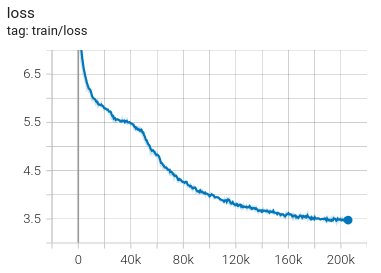
\includegraphics[width=0.6\textwidth]{figures/loss_inf_small.png}
	\caption{Loss Function during Training with Infineon Dataset and small trained tokenizer.}
	\label{fig:loss_small}
\end{figure}

\begin{figure}[H]
	\centering
	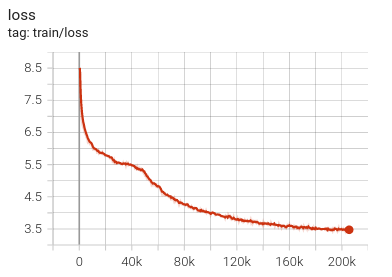
\includegraphics[width=0.6\textwidth]{figures/loss_inf_large.png}
	\caption{Loss Function during Training with Infineon Dataset and large trained tokenizer.}
	\label{fig:loss_large}
\end{figure}

\begin{figure}[H]
	\centering
	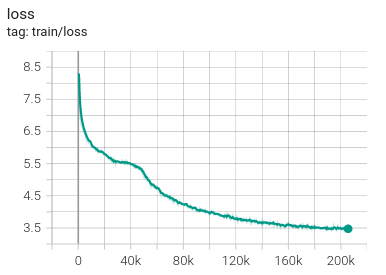
\includegraphics[width=0.6\textwidth]{figures/loss_inf_ext.png}
	\caption{Loss Function during Training with Infineon Dataset and extended tokenizer.}
	\label{fig:loss_ext}
\end{figure}

\begin{figure}[H]
	\centering
	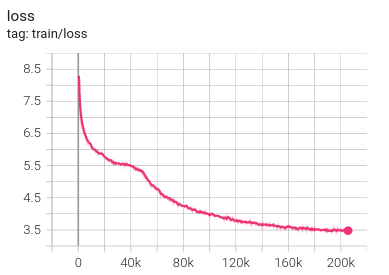
\includegraphics[width=0.6\textwidth]{figures/loss_infs2_s2.png}
	\caption{Loss Function during Training with tokenizer trained on s2.}
	\label{fig:loss_s2}
\end{figure}

\alert{Bild später ersetzen}
\begin{figure}[H]
	\centering
	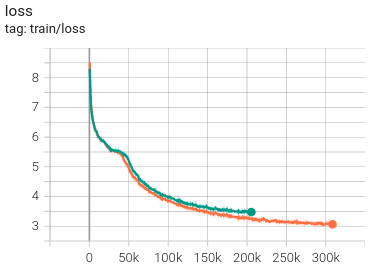
\includegraphics[width=0.6\textwidth]{figures/loss_infs2_large.png}
	\caption{Loss Function during Training with largest dataset and tokenizer trained on large.}
	\label{fig:loss_large_large}
\end{figure}

\alert{Hier Bild von gemeinsamen kurven einfügen}

The various loss functions hardly differ from each other. On the basis of the last curve, which was trained for 15 epochs, it can be seen that the longer training could certainly lead to a better performance. Nevertheless, the loss function already flattens out too much in this area. For this reason, further \alert{ measures} regarding the improvement of the training were researched.

\subsection{Trying different types of losses}
Another attempt to improve the performance of the model is to implement a different loss function. Cross entropy loss seemed to be particularly suitable. In the case of masked language modeling, this metric compares the token predicted by the model with the ground truth and assigns a value between 0 and 1 to the prediction. 0 stands for a perfect prediction. During training, the values are aggregated to represent the loss function. \newline
The loss function used by the \alert{Trainer object from Huggingface Transformers} is shown in Listing \ref{code:loss}.

\begin{code}
	\captionof{listing}{Trainer compute loss function}
	\label{code:loss}
\begin{minted}{python}
def compute_loss(self, model, inputs, return_outputs=False):
	if self.label_smoother is not None and "labels" in inputs:
		labels = inputs.pop("labels")
	else:
	labels = None
	outputs = model(**inputs)
	# Save past state if it exists
	if self.args.past_index >= 0:
		self._past = outputs[self.args.past_index]
	
	if labels is not None:
		loss = self.label_smoother(outputs, labels)
	else:
	# We don't use .loss here since the model may return tuples 
	# instead of ModelOutput.
	loss = outputs["loss"] if isinstance(outputs, dict) else outputs[0]
	
	return (loss, outputs) if return_outputs else loss
\end{minted}
\end{code}
\alert{quelle: https://github.com/huggingface/transformers/blob/v4.17.0/src/transformers/trainer.py#L2006}

which means that, by default, the model itself is responsible for computing some sort of loss and returning it to outputs. To implement an own loss function, we had to overwrite the Trainer class and the loss function and defining a cross entropy loss function to return it to outputs. The code is shown in listing \ref{code:cel}. We use the cross entropy loss function from \alert{torch.nn} here. In most cases the \alert{CrossEntropyLoss(}) function gets some weights as inputs, but because in our case pretraining a BERt model is an unsupervised learning task, we have no weights to assign and leave it empty.

\begin{code}
	\captionof{listing}{Cross Entropy Loss}
	\label{code:cel}
\begin{minted}{python}
class MyTrainer(Trainer):
	def compute_loss(self, model, inputs, return_outputs = False):
		labels = inputs.pop("labels")
		outputs = model(**inputs)
		logits = outputs.get("logits")

		loss_fct = nn.CrossEntropyLoss()
		loss = loss_fct(logits.view(-1, tokenizer.vocab_size),
				labels.view(-1))
		return (loss, outputs) if return_outputs else loss
\end{minted}
\end{code}

\subsection{Changing the Masking Method}
The original masking method which is used by all BERT based models is that every token in an input blocked gets masked by the probability of 15\%. 
\alert{hier fehlt noch was}

Based on the latest experiments, it can be seen that our models are not sufficiently well trained in the semiconductor area. Another attempt to improve the performance is to adjust the masking strategy during the training. After some research we came across the Whole Word Masking strategy. With this method, not only some tokens are randomly masked, but it is also checked whether the token to be masked is a standalone token or a subtoken. If a subtoken, which is part of a word, should get masked, the algorithm also masks all the surrounding tokens that belong to the word. In addition we increased the masking probability from 15\% to 20\%. The code is visible in Listing \ref{code:wwm}. Therefore we created a new data collator class \alert{which has the whole word masking method implemented} and handed this data collator to the trainer shown in Listing \ref{code:trainer_wwm}.

\alert{nicht vergessen tokenizer map funktion geändert damit word ids im dataset}
\begin{figure}[H]
	\centering
	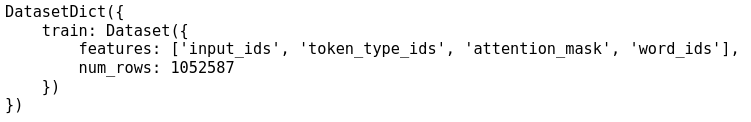
\includegraphics[width=0.6\textwidth]{figures/tok_dataset_wordids.png}
	\caption{Loss Function during Training with Infineon Dataset and large trained tokenizer.}
	\label{fig:data_wordids}
\end{figure}

\begin{code}
	\captionof{listing}{Data Collator implementing Whole Word Masking}
	\label{code:wwm}
\begin{minted}{python}
wwm_probability = 0.2

def whole_word_masking_data_collator(features):
	for feature in features:
	word_ids = feature.pop("word_ids")
	
	# Create a map between words and corresponding token indices
	mapping = collections.defaultdict(list)
	current_word_index = -1
	current_word = None
	for idx, word_id in enumerate(word_ids):
	if word_id is not None:
	if word_id != current_word:
	current_word = word_id
	current_word_index += 1
	mapping[current_word_index].append(idx)
	
	# Randomly mask words
	mask = np.random.binomial(1, wwm_probability, (len(mapping),))
	input_ids = feature["input_ids"]
	labels = feature["labels"]
	new_labels = [-100] * len(labels)
	for word_id in np.where(mask)[0]:
	word_id = word_id.item()
	for idx in mapping[word_id]:
	new_labels[idx] = labels[idx]
	input_ids[idx] = tokenizer.mask_token_id
	feature["labels"] = new_labels
	
	return torch_default_data_collator(features)
\end{minted}
\end{code}

\alert{Figure \ref{fig:wwm_ex} shows an example of how the whole word masking method works. The green examples shows how the algorithm is masking all surrounding subtokens which belong to a word were the blue example show some random picked tokens to mask which do not belong to any other word.}

\begin{figure}[H]
 	\centering
 	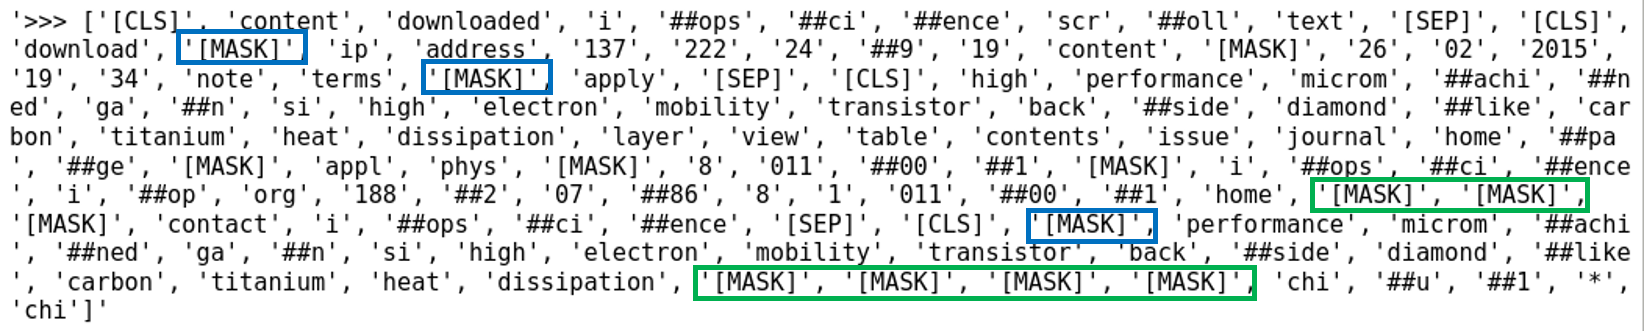
\includegraphics[width=1\textwidth]{figures/wwm_example.png}
 	\caption{Example of Whole Word Masking Method.}
 	\label{fig:wwm_ex}
 \end{figure}

\begin{code}
\captionof{listing}{Trainer}
\label{code:trainer_wwm}
\begin{minted}{python}
trainer = MyTrainer(
model=model.to(device),
args=training_args,
train_dataset=lm_datasets['train'],
data_collator=whole_word_masking_data_collator,
tokenizer=tokenizer
)
\end{minted}
\end{code}

We trained the model with the new masking method again for 20 epochs and the same learning rate and weight decay as in the other experiments. The results show a final loss of 2.51, which is the lowest loss in all experiments so far. The loss curve is depicted in Figure \ref{fig:loss_wwm}. This model could allow a good performance for the FA classifier after further training epochs. 

\begin{figure}[H]
	\centering
	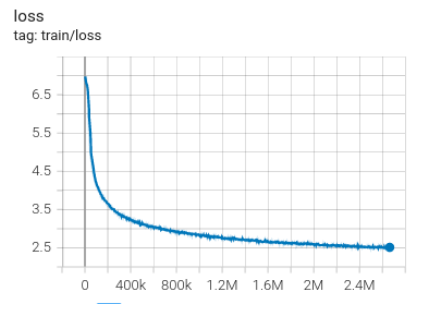
\includegraphics[width=0.6\textwidth]{figures/loss_wwm.png}
	\caption{Loss Function during Training with Whole Word Masking.}
	\label{fig:loss_wwm}
\end{figure}